\scanpage{7}
\mspage{\textcircled{3}}

% The upper calculations are canceled en bloc by three long oblique strokes
% and a sweeping left/bottom boundary. Each complete diagram, including its
% arrow paths, is wrapped in deleted; mbox keeps its drawing indivisible.
\[
\deleted{p_0p_{12}=p_0p_{13}=p_0\underbrace{p_{12}\rho^2}_{p_{31}}\sigma_2}
\qquad
\deleted{\rho^2\sigma_2=\sigma_3\rho^2}
\]
\diagram{\deleted{\mbox{\begin{tikzcd}[ampersand replacement=\&,row sep=small,column sep=large]
(x,y,z)\arrow[r,mapsto]\&(z,y,x)\&{}\\
{}\arrow[r]\&(x,z)\arrow[r]\&x
\end{tikzcd}}}}
\[\deleted{p_0p_{12}\sigma_1=p_0p_{12}}\]
\[\deleted{(x,x,y)}\]
% The continuation shaft has a separate tail bar and a small loop at its
% right endpoint. It is not replaced by the clear chevron of the row above.
\diagram{\deleted{\mbox{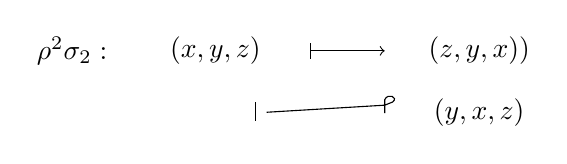
\begin{tikzpicture}[x=1cm,y=1cm]
\node[anchor=east] at (-0.8,0) {$\rho^2\sigma_2:$};
\node at (0.45,0) {$(x,y,z)$};
\node at (3.8,0) {$(z,y,x))$};
\draw[|->] (1.65,0)--(2.6,0);
\draw (0.96,-0.89)--(0.96,-0.65);
\draw (1.1,-0.78)--(2.6,-0.69);
\draw (2.6,-0.79)--(2.6,-0.62)
  .. controls (2.64,-0.53) and (2.78,-0.59) .. (2.7,-0.65)
  --(2.6,-0.69);
\node at (3.8,-0.78) {$(\uline{y,x},z)$};
\end{tikzpicture}}}}
\[
\begin{array}{ll}
\deleted{\delta_1\sigma=(x,y,y)}&{}\\[0.7ex]
\deleted{(x,\unsure{x},y)}&\qquad\deleted{z,x,y}\\[0.7ex]
\deleted{(y,y,x)}&{}
\end{array}
\]
% Tail bar and square downturned terminal are both visible; no chevron
% is supplied to the last coordinate mapping.
\diagram{\deleted{\mbox{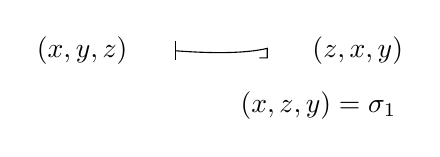
\begin{tikzpicture}[x=1cm,y=1cm]
\node at (0,0) {$(x,y,z)$};
\node at (3.5,0) {$(z,x,y)$};
\draw (1.18,-0.12)--(1.18,0.12);
\draw (1.18,0) .. controls (1.7,-0.04) and (2.1,-0.03) .. (2.35,0.03)
  --(2.35,-0.09)--(2.25,-0.09);
\node at (3.0,-0.7) {$(x,z,y)=\sigma_1$};
\end{tikzpicture}}}}

\mspage{\textcircled{3}}
Si $E_0$ est réduit à un p\textsuperscript{t}, donc par $\delta_0,\delta_1\delta_0$ $E_1,E_2$ deviennent des ens. pointés, et $\mathcal G_2,\mathcal G_3$ respectent la ponctuation.
\margin{(``ponctués'')}
\deleted{\unsure{Donc.|On a.}}
$\deleted{\delta_1}$ \deleted{respecte \unsure{les|le}}
Donc, en plus des opérations de $\mathcal G_2,\mathcal G_3$, on a
\diagram{\begin{tikzcd}[ampersand replacement=\&,column sep=large]
E_1\arrow[r,bend right=35,"\delta_1"']\&E_2\arrow[l,"p_{12}"']
\end{tikzcd}}
, où $\delta_1$ \inserted{et $p_{12}$} respect\unsure{ent}%
% The terminal low loop, high arch and return touch the right paper edge;
% the compressed n/t cannot be separated securely. No punctuation supplied.
\ les ponctuations, et où $p_{12},\delta_1$ satisfont aux cinq relations supplémentaires
\[\boxed{\begin{aligned}
p_{12}\delta_1&=\sigma\\
p_{12}\underbrace{\rho\delta_1}_{\delta_3}&=\text{application constante de valeur }e_1\quad\text{(p\textsuperscript{t} marqué de }E_1\text{)}\\
p_{12}\underbrace{\rho^2\delta_1}_{\delta_2}&=\mathrm{id}_{E_1}\\
\sigma_1\delta_1&=\delta_1\\
p_{12}\sigma_3&=\sigma p_{12}
\end{aligned}}\]
% This smaller compartment sits inside the lower right of the outer box,
% sharing its right and bottom boundary; the following marginal items are
% adjacent to its three rows. Their textual state is preserved separately.
\margin{$\boxed{\begin{aligned}
p_{12}\delta_2&=\mathrm{id}_{E_1}\\
p_{12}\underbrace{\rho\delta_2}_{\delta_1}&=\sigma\\
p_{12}\underbrace{\rho^2\delta_2}_{\delta_3}&=e_1\quad\text{(application de }E_1\text{ sur }e_1\text{)}
\end{aligned}}$}
\margin{$\uline{p_{12}\sigma_3=\sigma p_{11}}$\\
$\sigma_2\delta_2=\delta_2$\\
$\deleted{p_{12}\sigma_3\unsure{=\sigma}p_{12}}$\\
$\deleted{\unsure{\mathrm{id}}}$\\
\begin{tikzcd}[ampersand replacement=\&,column sep=large]
E_1\arrow[r,bend right=12,"\delta_1"']\&E_2\arrow[l,"p_{12}"']
\end{tikzcd}}
\margin{6}
